% use sigconf format
\documentclass[sigconf]{acmart}

\usepackage{subcaption}
\usepackage[ruled,linesnumbered,commentsnumbered]{algorithm2e}

\let\oldnl\nl% Store \nl in \oldnl
\newcommand{\nonl}{\renewcommand{\nl}{\let\nl\oldnl}}% Remove line number for one line

\newcommand{\minof}[1]{#1_{\text{min}}}
\newcommand{\maxof}[1]{#1_{\text{max}}}

\SetCommentSty{textit}

% hide copyright & ACM reference
\setcopyright{none}
\settopmatter{printacmref=false}
\renewcommand\footnotetextcopyrightpermission[1]{}
\citestyle{acmnumeric}
\setcitestyle{numbers,sort}

\begin{document}

\title{Parallelization of Regular Expression Matching}

\author{Jun-Yao Jiang}
\affiliation{%
	\institution{National Yang Ming Chiao Tung University}
	\city{Hsinchu}
	\country{Taiwan}
}
\authornote{All authors contributed equally to this research.}
\email{audi15420.cs10@nycu.edu.tw}


\author{Pin-Wen Chen}
\affiliation{%
	\institution{National Yang Ming Chiao Tung University}
	\city{Hsinchu}
	\country{Taiwan}
}
\authornotemark[1]
\email{nc.110550144.cs10@nycu.edu.tw}


\author{Ren-Hao Deng}
\affiliation{%
	\institution{National Yang Ming Chiao Tung University}
	\city{Hsinchu}
	\country{Taiwan}
}
\authornotemark[1]
\email{ddeng.cs10@nycu.edu.tw}

% abstract
\begin{abstract}
	This work explores parallelizing deterministic finite automata (DFA) matching for regular expression processing to enhance computational efficiency. By addressing the limitations of conventional enumeration methods—namely, the high overhead from unknown initial states—a novel approach inspired by Pararegex is implemented. This method tracks active states dynamically, significantly reducing redundant computations. Further optimizations involve CUDA for leveraging massive thread parallelism and advanced memory management techniques. Experimental results demonstrate improved speedups across varying input lengths, thread counts, and state numbers, highlighting the effectiveness of combining OpenMP and CUDA with active state tracking in reducing computational overhead.
\end{abstract}

% generate the title, authors, and abstract
\pagestyle{plain}
\maketitle

% main sections
\section{Introduction}

Regular Expressions (regex) are powerful tools for searching, matching, and manipulating strings based on specific patterns. They are essential in fields such as programming, text processing, and data validation.

The conventional approach to serial matching of regex rules involves transforming these expressions into Nondeterministic Finite Automata (NFA) or Deterministic Finite Automata (DFA). Traditional enumeration-based parallel methods typically divide input strings into segments, assigning each segment to different threads. However, this process may result in the initial state of each segment except for the first one being unknown, which can introduce significant computational overhead.

In their work, Zhe Fu et al. \cite{pararegex} introduced a novel method for parallelizing regex that reduces overhead by implementing a new structure, referred to as the Middle State Unit (MSU). Their approach demonstrates an impressive speedup of up to six times when combined with Delayed Input DFA on an Intel Core i7-4790 CPU, which features four cores and eight threads. In this project, we aim to implement the enumeration method and various improvement techniques, such as this one, subsequently comparing the results with those obtained from a serial implementation.

\section{Proposed Solution}

In this section, we detail the methodologies employed to improve the efficiency of regular expression matching through various parallelization techniques. These include enumeration, Pararegex, basic CUDA optimization, advanced CUDA strategies, and a combined CUDA and OpenMP approach.

\subsection{Enumeration}
We reference the enumeration \cite{enumeration} algorithm address in Algorithm~\ref{alg:enumeration} in this part. The basic idea behind parallelization through enumeration is to divide the input text into segments, process each segment with a separate thread running the automaton, and then combine the results in the main thread. However, the problem comes with joining the results, as the initial state of each segment except for the first one is unknown. If each segment needs to wait for the last segment to finish, it'll become a serial process. To solve this problem, the enumeration method considers all states as initial states, finds all corresponding last active states for each, and joins all subresults sequentially. This exhaustive approach introduces significant computational overhead proportional to the number of states, as the calculation must account for almost (\emph{state count})x computations. The Big-O complexity is therefore expressed as:

\[
	O\left(\frac{|Q|n}{|P|} + \log |P| + |P|\right)
\]

where $n$ is the input string length, $|P|$ is the number of processors, and $Q$ is the number of states. In scenarios when $n \gg |P|$, the terms $\log |P|$ and $|P|$ can be ignored, simplifying the expression to:

\[
	O\left(\frac{|Q|n}{|P|}\right)
\]

The speedup is calculated as the input length $n$ divided by the computation time, resulting in $O\left(\frac{|P|}{|Q|}\right)$. This indicates that the speedup is directly proportional to the number of processors $|P|$ and inversely proportional to the number of states $Q$.

This limitation highlights a critical problem: the enumeration method's performance is significantly hindered by the number of states. Is there a way to solve this problem? This brings us to the next section, Pararegex.

\begin{algorithm}
	\KwIn{A transition table $T$, set of final states $\mathcal{F}$, mapping from possible initial state to possible last visited state $\mathcal{L}$, and input text $t = t_1 t_2 \dots t_n$.}
	\KwOut{Output of run of DFA}
	\nonl\textbf{Method:}
	Each processor $P_i$ has a unique number. The total number of processors is $|P|$. The size of DFA is $|Q|$.

	\SetKwBlock{Begin}{begin}{end}
	\Begin{
	\ForEach{$P_i \in [P_0,P_1,\cdots,P_{|P|-1}]$ \textit{parallel}}{
	$\text{start\_pos} \gets \lfloor{P_i\frac{n}{|P|}}\rfloor$ \;
	$\text{end\_pos} \gets \lfloor{(P_i+1)\frac{n}{|P|}}\rfloor-1$ \;
	\For{$j = 0 \to |Q| - 1$}{
		$\mathcal{L}[P_i][j] \gets j$ \tcp*{Initialize $\mathcal{L}$ vector}
		\For{$k \gets \text{start\_pos}$ \KwTo $\text{end\_pos} - 1$}{
			$t_k \gets t[k]$ \;
			$\mathcal{L}[P_i][j] \gets T[\mathcal{L}[P_i][j], t_k]$ \tcp*{Evaluate transition}
			\If{$\mathcal{L}[P_i][j] = -1$}{
				\textbf{break} \;
			}
		}
	}
	}
	\#pragma omp barrier \tcp{Wait for the slowest processor}
	$\text{result} \gets \textbf{perform\_parallel\_reduction()}$\;
	}
	\caption{Enumeration implementation}
	\label{alg:enumeration}
\end{algorithm}

\subsection{Pararegex}
We reference the Pararegex \cite{pararegex} algorithm described in Algorithm~\ref{alg:pararegex} to mitigate the overhead caused by the DFA huge states number. Our initial implementation uses OpenMP.

Similar to enumeration, in each thread (except the first thread), we consider all DFA states as potential starting states. However, unlike traditional enumeration methods, as input is gradually processed, we record the states transitioned to as ``active states''. Instead of enumerating through all DFA states for all input processed by the threads, we only focus on these active states, as they are the only ones capable of matching the given input. Since DFA transitions are many-to-one, we expect the number of ``active states'' to decrease over time, shown in Theorem~\ref{thm:active_states} due to \cite{pararegex}. According to the paper's statistics, after processing just one character, the number of active states can drop to about 1\% of the original number of states. Therefore, if we can efficiently track these active states after each input during the mapping and matching phases, the state overhead present in the original enumeration method will be significantly reduced due to the dramatic decrease in active states.

\begin{theorem}
	Let $Q_0$ be the set of all states of DFA $D$, and $Q_m$ be the set of active DFA states after reading $m$ input characters when all DFA states are active as start states. Then, for all $0 \leq i < j \leq m$, we have $|Q_i| \geq |Q_j|$.
	\label{thm:active_states}
\end{theorem}

\begin{proof}
	Assume that $\exists\ 0 \leq i < j \leq m$ s.t. $|Q_i| < |Q_j|$. Then, there must $\exists\ k, i \leq k < k+1 \leq j$ s.t. $|Q_k| < |Q_{k+1}|$. This means that there must exist at least one DFA state, say $\hat{q}$, s.t. $|\delta (\hat{q})| > 1$. This contradicts the fact that the transition function $\delta$ of DFA only takes and returns a single state, thus contradicting the assumption.
\end{proof}

The paper proposes an MSU method for managing active states during the mapping and matching procedures (Figure~\ref{fig:Pararegex_1}). Each MSU consists of a state ID and is associated with a one-hot bit vector called the ``mapping vector''. The vector is initialized with the ID's bit set to one, indicating that the current state (ID) can transition from any state where the corresponding bit in the mapping vector is set to one. After processing an input character, if two MSUs transition to the same active state, they are merged into a single one. The state ID is updated to the resulting active state, and their mapping vectors are combined using a bitwise OR operation. This represents that the new active state can transition from any states that transitioned to the two original states in response to the previous input character.

We can infer that after each thread processes its input partition, each thread will retain a few MSUs, ideally just one, representing the active states matching the input partition of that thread. The result is reduced starting from the first thread's final state (the first thread begins with only the start state, so it has only one MSU; see Figure~\ref{fig:Pararegex_2}). An AND operation is performed between the MSUs retained by the current thread and the next thread. If the output of the AND operation is one, it indicates that the active state ID of the MSU can be transitioned from the final state of the previous thread. This process continues, reducing the states at each step, until the final thread. At this point, we obtain the final state after reading the entire input and checking whether it belongs to the set of accepting states.

In time complexity analysis, the initialization takes $O(\left| Q \right|)$, the matching and mapping procedure takes $O\left(\frac{|Q_{\text{active}}|n}{|P|}\right)$, the union procedure takes $O(n^2)$ since in the implementation, \textbf{we find C++ map is broken}, and array access overhead is more than squared reduction for the number of active states is usually very small, and the reduction procedure takes $O(|P|)$. The overall time complexity is $O\left( \frac{|Q_{\text{active}}|n}{|P|} + |Q| + |Q_{\text{active}}|^2 + |P| \right)$, as n large enough, become $O\left( \frac{|Q_{\text{active}}|n}{|P|} \right)$. From both the paper's findings and our statistical analysis, we can expect |Q| to decrease rapidly. In the best case, the algorithm achieves $O(|P|)$ speedup, which also aligns with the average-case performance in our analysis. This approach effectively resolves the inefficiency in enumeration.

\begin{algorithm}
	\KwIn{Pararegex $P =\{M, \Sigma, \delta, M_0, F_M\}$, input $C = c_{11}c_{12}\cdots c_{1m_1}c_{21}\cdots c_{2m_2}c_{n1}\cdots c_{nm_n}$, number of threads $n$}
	\KwOut{$q_{final}$}
	\tcp{mapping and matching procedure;}
	\ForEach{$i \in [1 \dots n]$ \textit{parallel}}
	{
		\eIf{$i = 1$}
		{
			$M_i \gets q_0$\;
		}{
			$M_i \gets M_0$\;
		}
		\For{$j = 1 \to m_i$}
		{
			\ForEach{$msu \in M_i$}
			{
				$msu \gets \delta(msu,c_{ij})$
			}
			merge $MSUs$ with the same $msu.id$
		}
	}
	\tcp{reducing procedure;}
	$msu_{final} \gets M_i$
	\For{$i = 2 \to n$}
	{
		\ForEach{$msu \in M_i$}
		{
			\If{$msu_{final}.id \&\& msu.mapping \ne 0$}
			{
				$msu_{final}.id \gets msu.id$
			}
		}
	}
	$q_{final} \gets msu_{final}.id$
	\caption{Pararegex implementation}
	\label{alg:pararegex}
\end{algorithm}

\begin{figure*}[t]
	\begin{subfigure}{.6\textwidth}
		\centering
		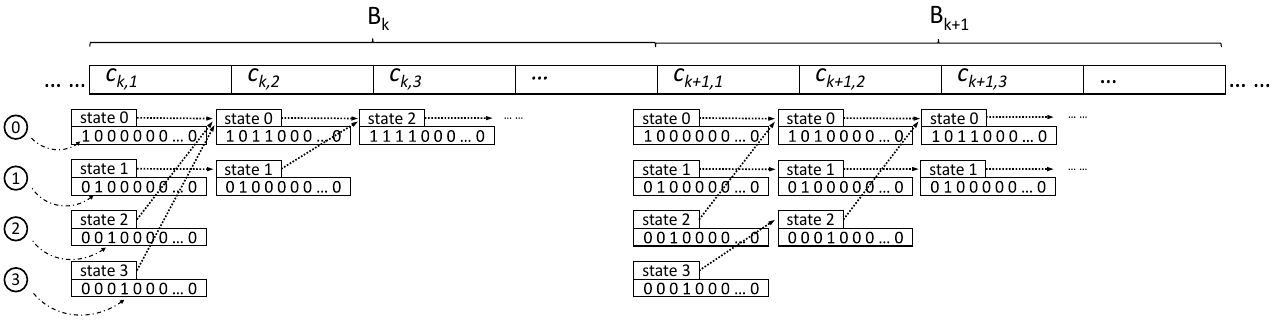
\includegraphics[width=\linewidth]{Pararegex_1}
		\caption{}
		\label{fig:Pararegex_1}
	\end{subfigure}
	\begin{subfigure}{.3\textwidth}
		\centering
		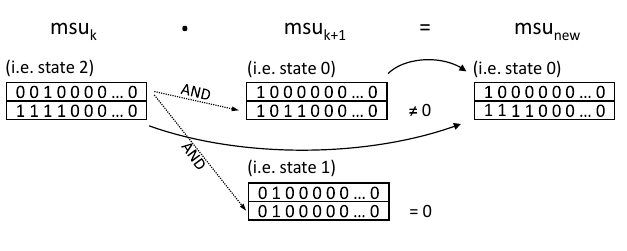
\includegraphics[width=\linewidth]{Pararegex_2}
		\caption{}
		\label{fig:Pararegex_2}
	\end{subfigure}
	\caption{Pararegex: (a) Mapping and matching procedure with MSUs, (b) Reducing procedure}
\end{figure*}

\subsection{Basic CUDA Implementation}
In the previous part, we know that the original enumeration approach has the speedup of $O\left(\frac{|P|}{|Q|}\right)$, which $|P|$ means the input text is split into $|P|$ segments.

Now, this basic CUDA implementation extends the enumeration approach to utilize the vast parallelism offered by GPUs. By assigning input segments to CUDA threads, this method leverages the high number of CUDA cores for concurrent processing. This means we set $|P| = |P_{\text{cuda}}|$, which $|P_{\text{cuda}}|$ means the number of processors made by CUDA on our GPU, and the speedup is modified to be $O\left(\frac{|P_{cuda}|}{|Q|}\right)$. However, it suffers from significant memory overhead due to the large number of states and frequent global memory access.

\subsection{Advanced CUDA Implementation}
In advanced CUDA implementation, we similarly transfer the DFA, input, and a mapping table of size $|Q| \times |P|$ (used to store enumeration results) to the device's global memory due to size constraints.

Unlike the basic implementation, we expand CUDA threads not only across processors but also along the state dimension. Specifically, we assign each thread a slightly longer input sequence but make it responsible for only one state. Instead of setting $|P| = |P_{\text{cuda}}|$ as in previous method, we set $|P| = \frac{|P_{\text{cuda}}|}{|Q|}$ since we need a CUDA thread per state. Although the speedup remains the same, i.e.,$O\left(\frac{|P_{cuda}|}{|Q|}\right)$, this approach reduces the number of memory accesses for state output by a factor of $|Q|$ per CUDA thread, as discussed below.

A detailed analysis of the memory access patterns yields the following insights:

\begin{itemize}
	\item \textbf{Input Memory Access:} In the basic implementation, the total input memory access per thread is given by
	      \[
		      \left(\frac{n}{|P|}\right) \times |Q| = \left(\frac{n}{|P_{\text{cuda}}|}\right) \times |Q| = \frac{n|Q|}{|P_{\text{cuda}}|}
	      \]
	      where $n$ represents the length of the input string, and $|P|$ is the number of input partitions. In contrast, the advanced method can be expressed as
	      \[
		      \left(\frac{n}{|P|}\right) = \frac{n}{\left(\frac{|P_{\text{cuda}}|}{|Q|}\right)} = \frac{n|Q|}{|P_{\text{cuda}}|}
	      \]
	      Despite differences in the access patterns, both methods result in the same total input memory access.

	\item \textbf{DFA Memory Access:} In the basic implementation, the total DFA memory access per thread is
	      \[
		      |Q| \times \left(\frac{n}{|P|}\right) = |Q| \times \left(\frac{n}{|P_{\text{cuda}}|}\right) = \frac{n|Q|}{|P_{\text{cuda}}|}
	      \]
	      While in the advanced method, it is
	      \[
		      \left(\frac{n}{|P|}\right) = \frac{n}{\left(\frac{|P_{\text{cuda}}|}{|Q|}\right)} = \frac{n|Q|}{|P_{\text{cuda}}|}
	      \]
	      Similar to input memory access, both methods incur the same total DFA memory access.

	\item \textbf{State Output Memory Access:} In the basic implementation, each thread accesses the state output $2 \times |Q|$ times, to both read and write the results. In contrast, the advanced method reduces this to only two accesses per thread—one for reading and one for writing—leading to a significant reduction in overhead.
\end{itemize}

These results highlight that the advanced method capitalizes on register memory to store state data, whereas the basic implementation relies more heavily on global memory. By  minimizing global memory accesses, the advanced method optimizes overall performance. The observed improvements are primarily attributed to reducing memory access overhead on state output memory access and more efficient use of CUDA threads.

\subsection{Advanced CUDA + OpenMP}
We observed that state overheads persist in advanced CUDA enumeration. To address this, we attempted to integrate the concept of active states from Pararegex\cite{pararegex}. By reducing the number of states enumerated in CUDA, each thread could handle a shorter input partition, leading to less conflict in memory access for both the input and possibly the DFA.

To achieve this, we first use Pararegex in OpenMP to reduce the number of states. However, during implementation, we discovered a significant difference in efficiency between reducing states for one character and simulating states for two characters. When reducing for one character, the number of states can drop to an average of 10\% of the original DFA states. Furthermore, it is possible to precompute the corresponding initial states for one character reduction.

While two-character reduction can also be precomputed, it requires quadratic time complexity. Additionally, using OpenMP to simulate two characters for a CUDA-level number of threads results in overheads that outweigh the benefits of the reduced state count compared to one character. As a result, we adopted the one-character reduction approach.

Ultimately, we found that this reduction technique could also be applied to OpenMP-based Pararegex. However, since OpenMP-based Pararegex dynamically reduces the active states with each input character, the resulting state count is already significantly smaller. Consequently, this reduction technique does not substantially contribute to the overall speedup of OpenMP-based Pararegex.


\section{Experimental Methodology}
In this section, we outline the experimental methodology used to evaluate the performance of various matching techniques. We first present the framework, followed by discussing the implementations and evaluation metrics.

\subsection{Framework}

The proposed framework is illustrated in Figure~\ref{fig:Framework}. This framework is designed to evaluate the performance of various matching techniques implemented for detecting network intrusions based on Snort community rules \cite{snortRules}. Initially, the regular expression patterns from the Snort rules are filtered and converted into a minimized DFA. These minimized DFAs are subsequently utilized by matchers to evaluate input strings formed by concatenating packet payloads from the DARPA dataset \cite{DARPA}.


\begin{figure}[t]
	\centering
	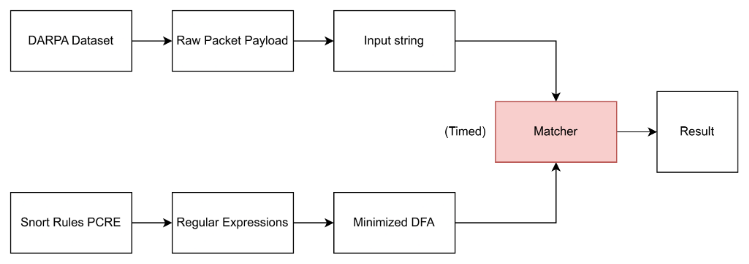
\includegraphics[width=\linewidth]{framework}
	\caption{Framework Overview}
	\Description{The framework first filters regular expressions derived from Snort community rules and converts them into minimized DFAs. These DFAs are then used by matchers to process input strings created from concatenated packet payloads in the DARPA dataset.}
	\label{fig:Framework}
\end{figure}

\subsection{Baseline}

The baseline for performance comparison is established using a serial implementation of the matching algorithm. In this approach, the algorithm begins from the initial state of the DFA and processes each input character sequentially. Once the entire input string has been consumed, the algorithm checks whether the current state is an accepting state to determine if a match has been found. The result is then recorded for subsequent validation against the other methods.

\subsection{Optimization Approaches}

The enumeration method is implemented using OpenMP to give us an insight into the potential speedup achieved by distributing the input string across multiple threads. Following this, the aforementioned methods outlined below are applied to optimize performance further:

\begin{itemize}
	\item \textbf{Pararegex:} Implements MSUs to track active states, thereby reducing the initial state overhead introduced by the enumeration method.
	\item \textbf{Basic CUDA:} Leverages the high degree of parallelism offered by GPUs to accelerate the enumeration method.
	\item \textbf{Advanced CUDA:} Enhances memory access patterns through parallelizing states on the CUDA platform.
	\item \textbf{Advanced CUDA + OpenMP:} Combines OpenMP for an initial iteration of the Pararegex method before passing the results to CUDA for further processing.
\end{itemize}

Along with verifying the correctness of the methods, the execution times will be compared to the baseline in order to quantify the speedup achieved by each optimization.

\subsection{Evaluation Metrics}

The performance of the proposed methods is evaluated in terms of speedup, using the following three variables:

\begin{itemize}
	\item \textbf{Input Length:} The size of the input packet payloads is varied to examine how each method scales with larger datasets, ranging from $10^3$ to $10^9$.
	\item \textbf{Number of States:} The number of states in the DFA is varied across five configurations to find out how the complexity of the matching process impacts performance and to investigate the effect of the ``active state'' mechanism on optimization.
	\item \textbf{(CPU) Number of Threads:} The number of threads used for parallel processing with OpenMP is varied to analyze the impact of CPU parallelism on performance, ranging from 1 to 12.
\end{itemize}

Unless specified as a variable, the following parameters are fixed: input length = $10^9$, number of states = 79, and number of threads = 4.

\section{Experimental Result}

The experimental evaluation was conducted on a system featuring an Intel(R) Core(TM) i7-8700K CPU (6 cores, 12 threads) at 3.70GHz, 64GB DDR4 RAM, and an NVIDIA RTX 4090 GPU with 24GB memory.

\begin{figure*}[t]
	\begin{subfigure}{.33\textwidth}
		\centering
		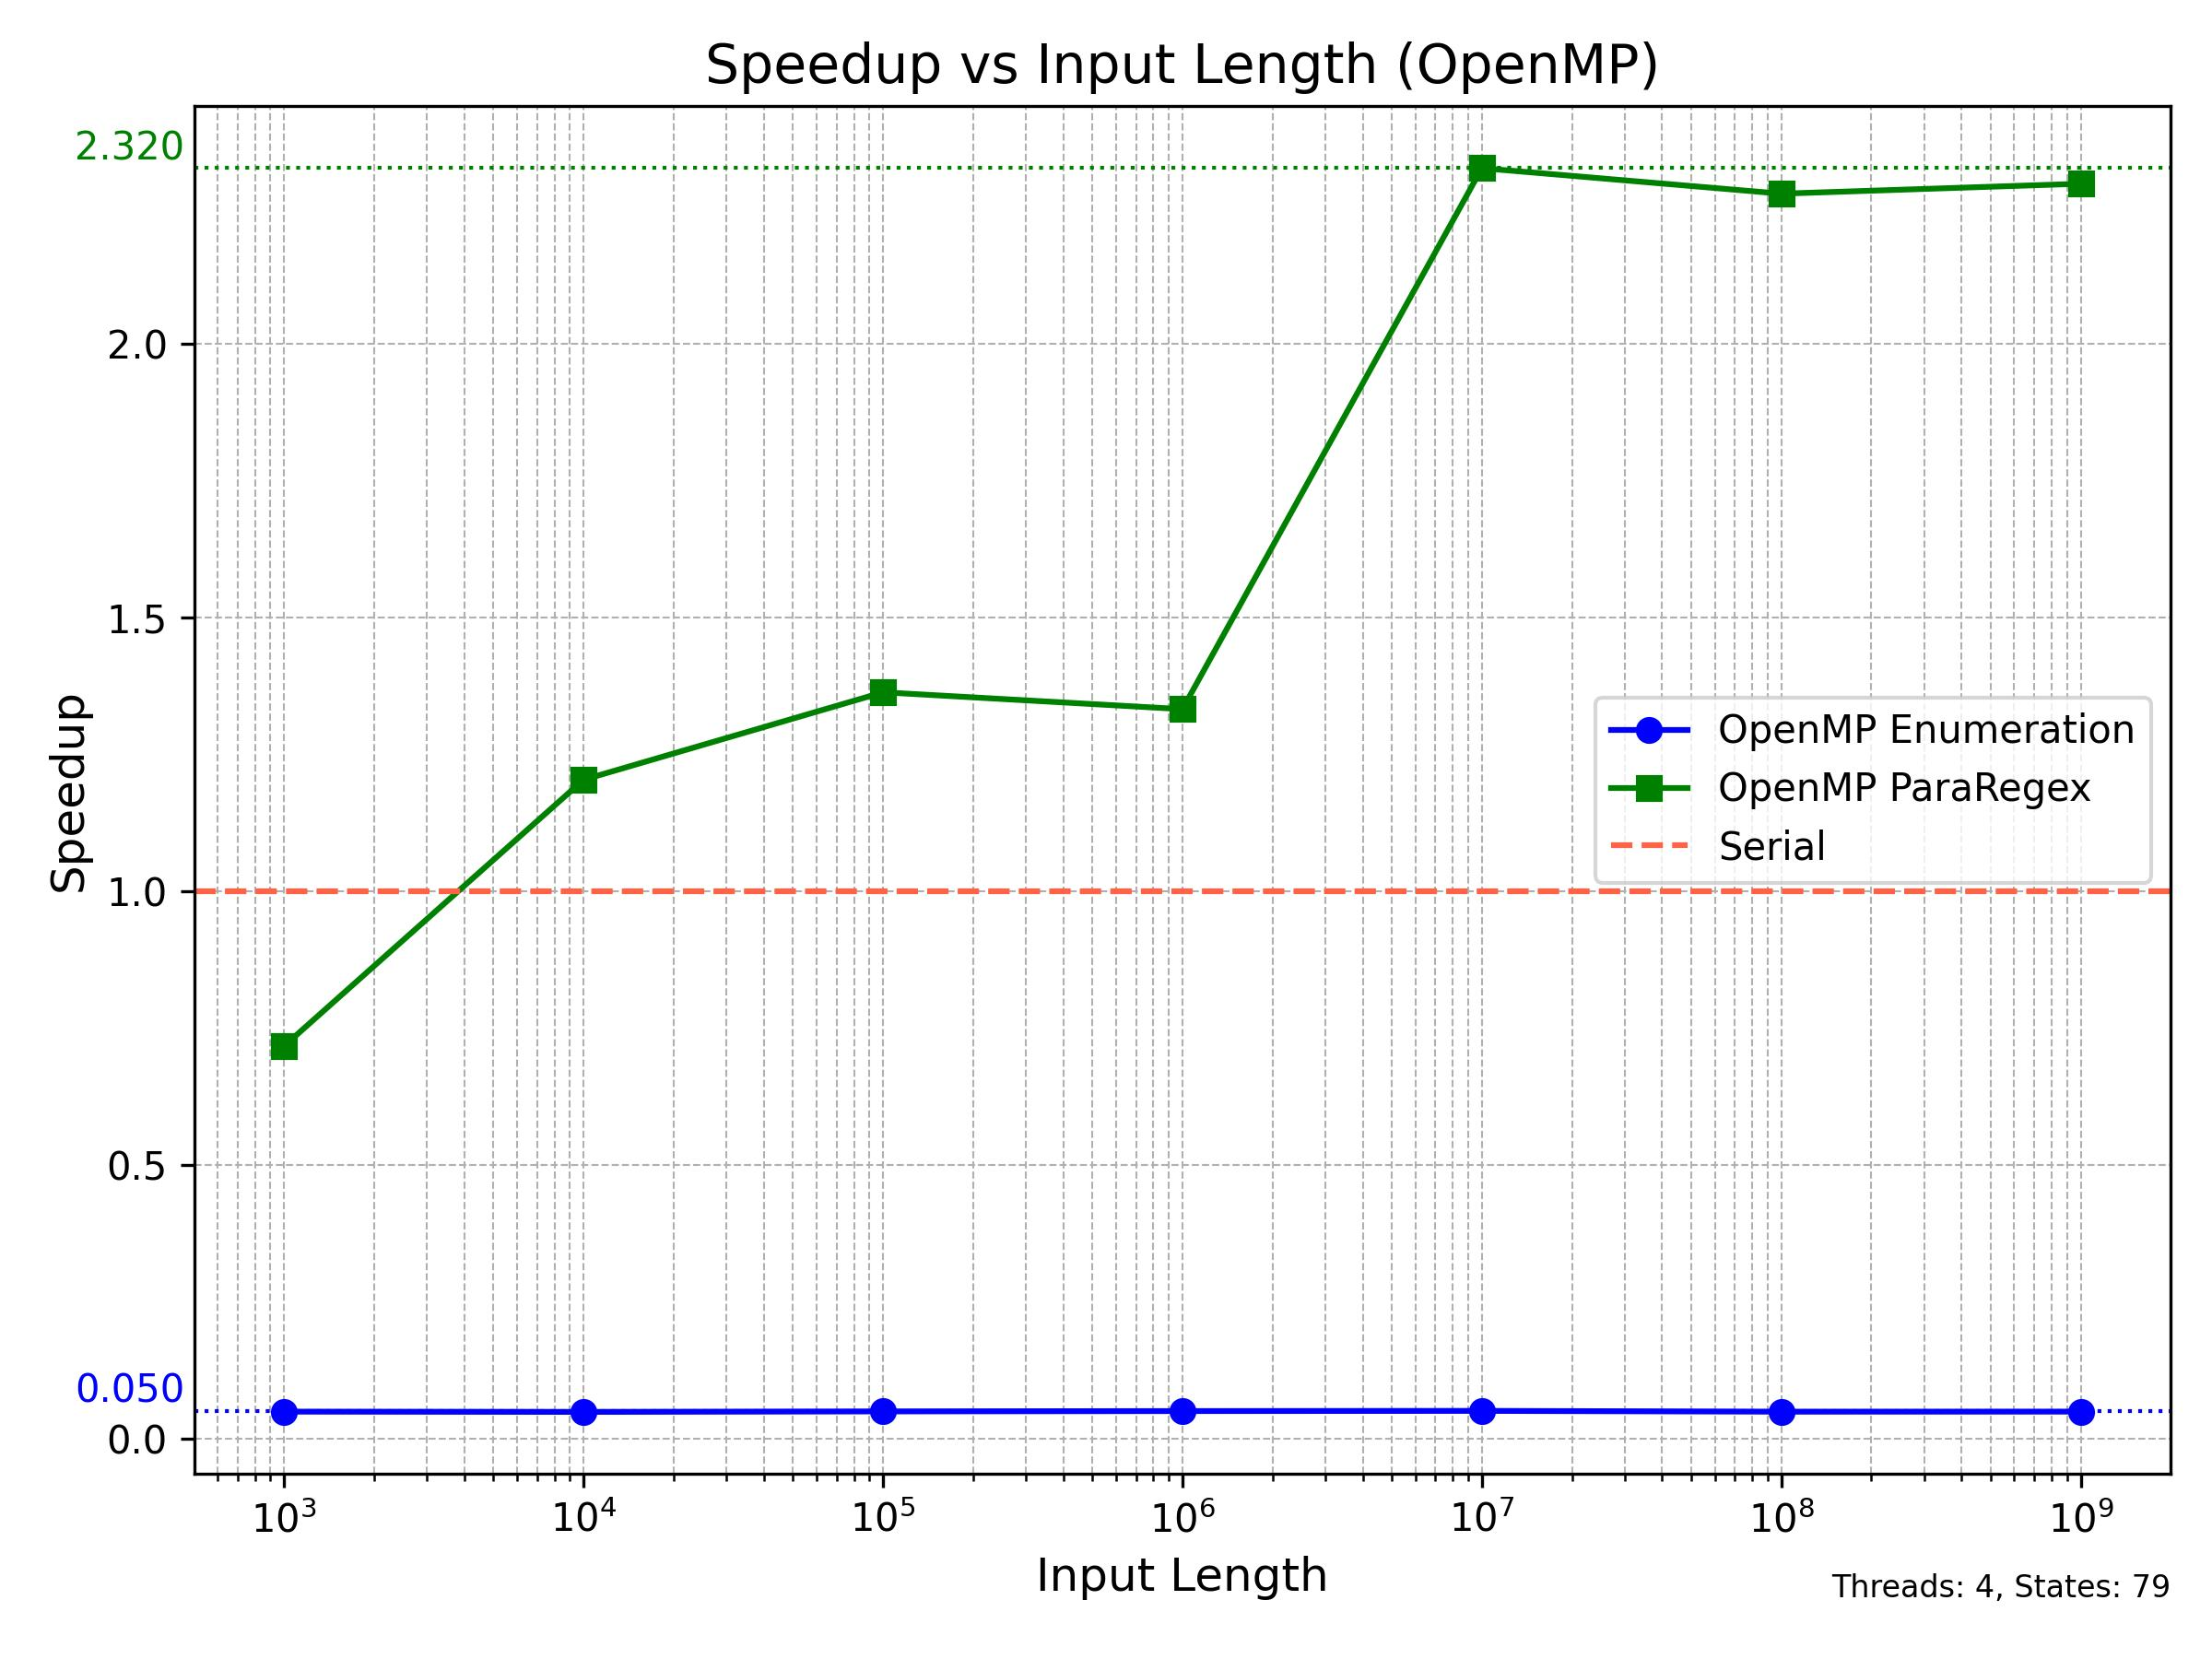
\includegraphics[width=\linewidth]{input_length_omp}
		\caption{}
		\label{fig:SpeedupInputLengthOMP}
	\end{subfigure}
	\begin{subfigure}{.33\textwidth}
		\centering
		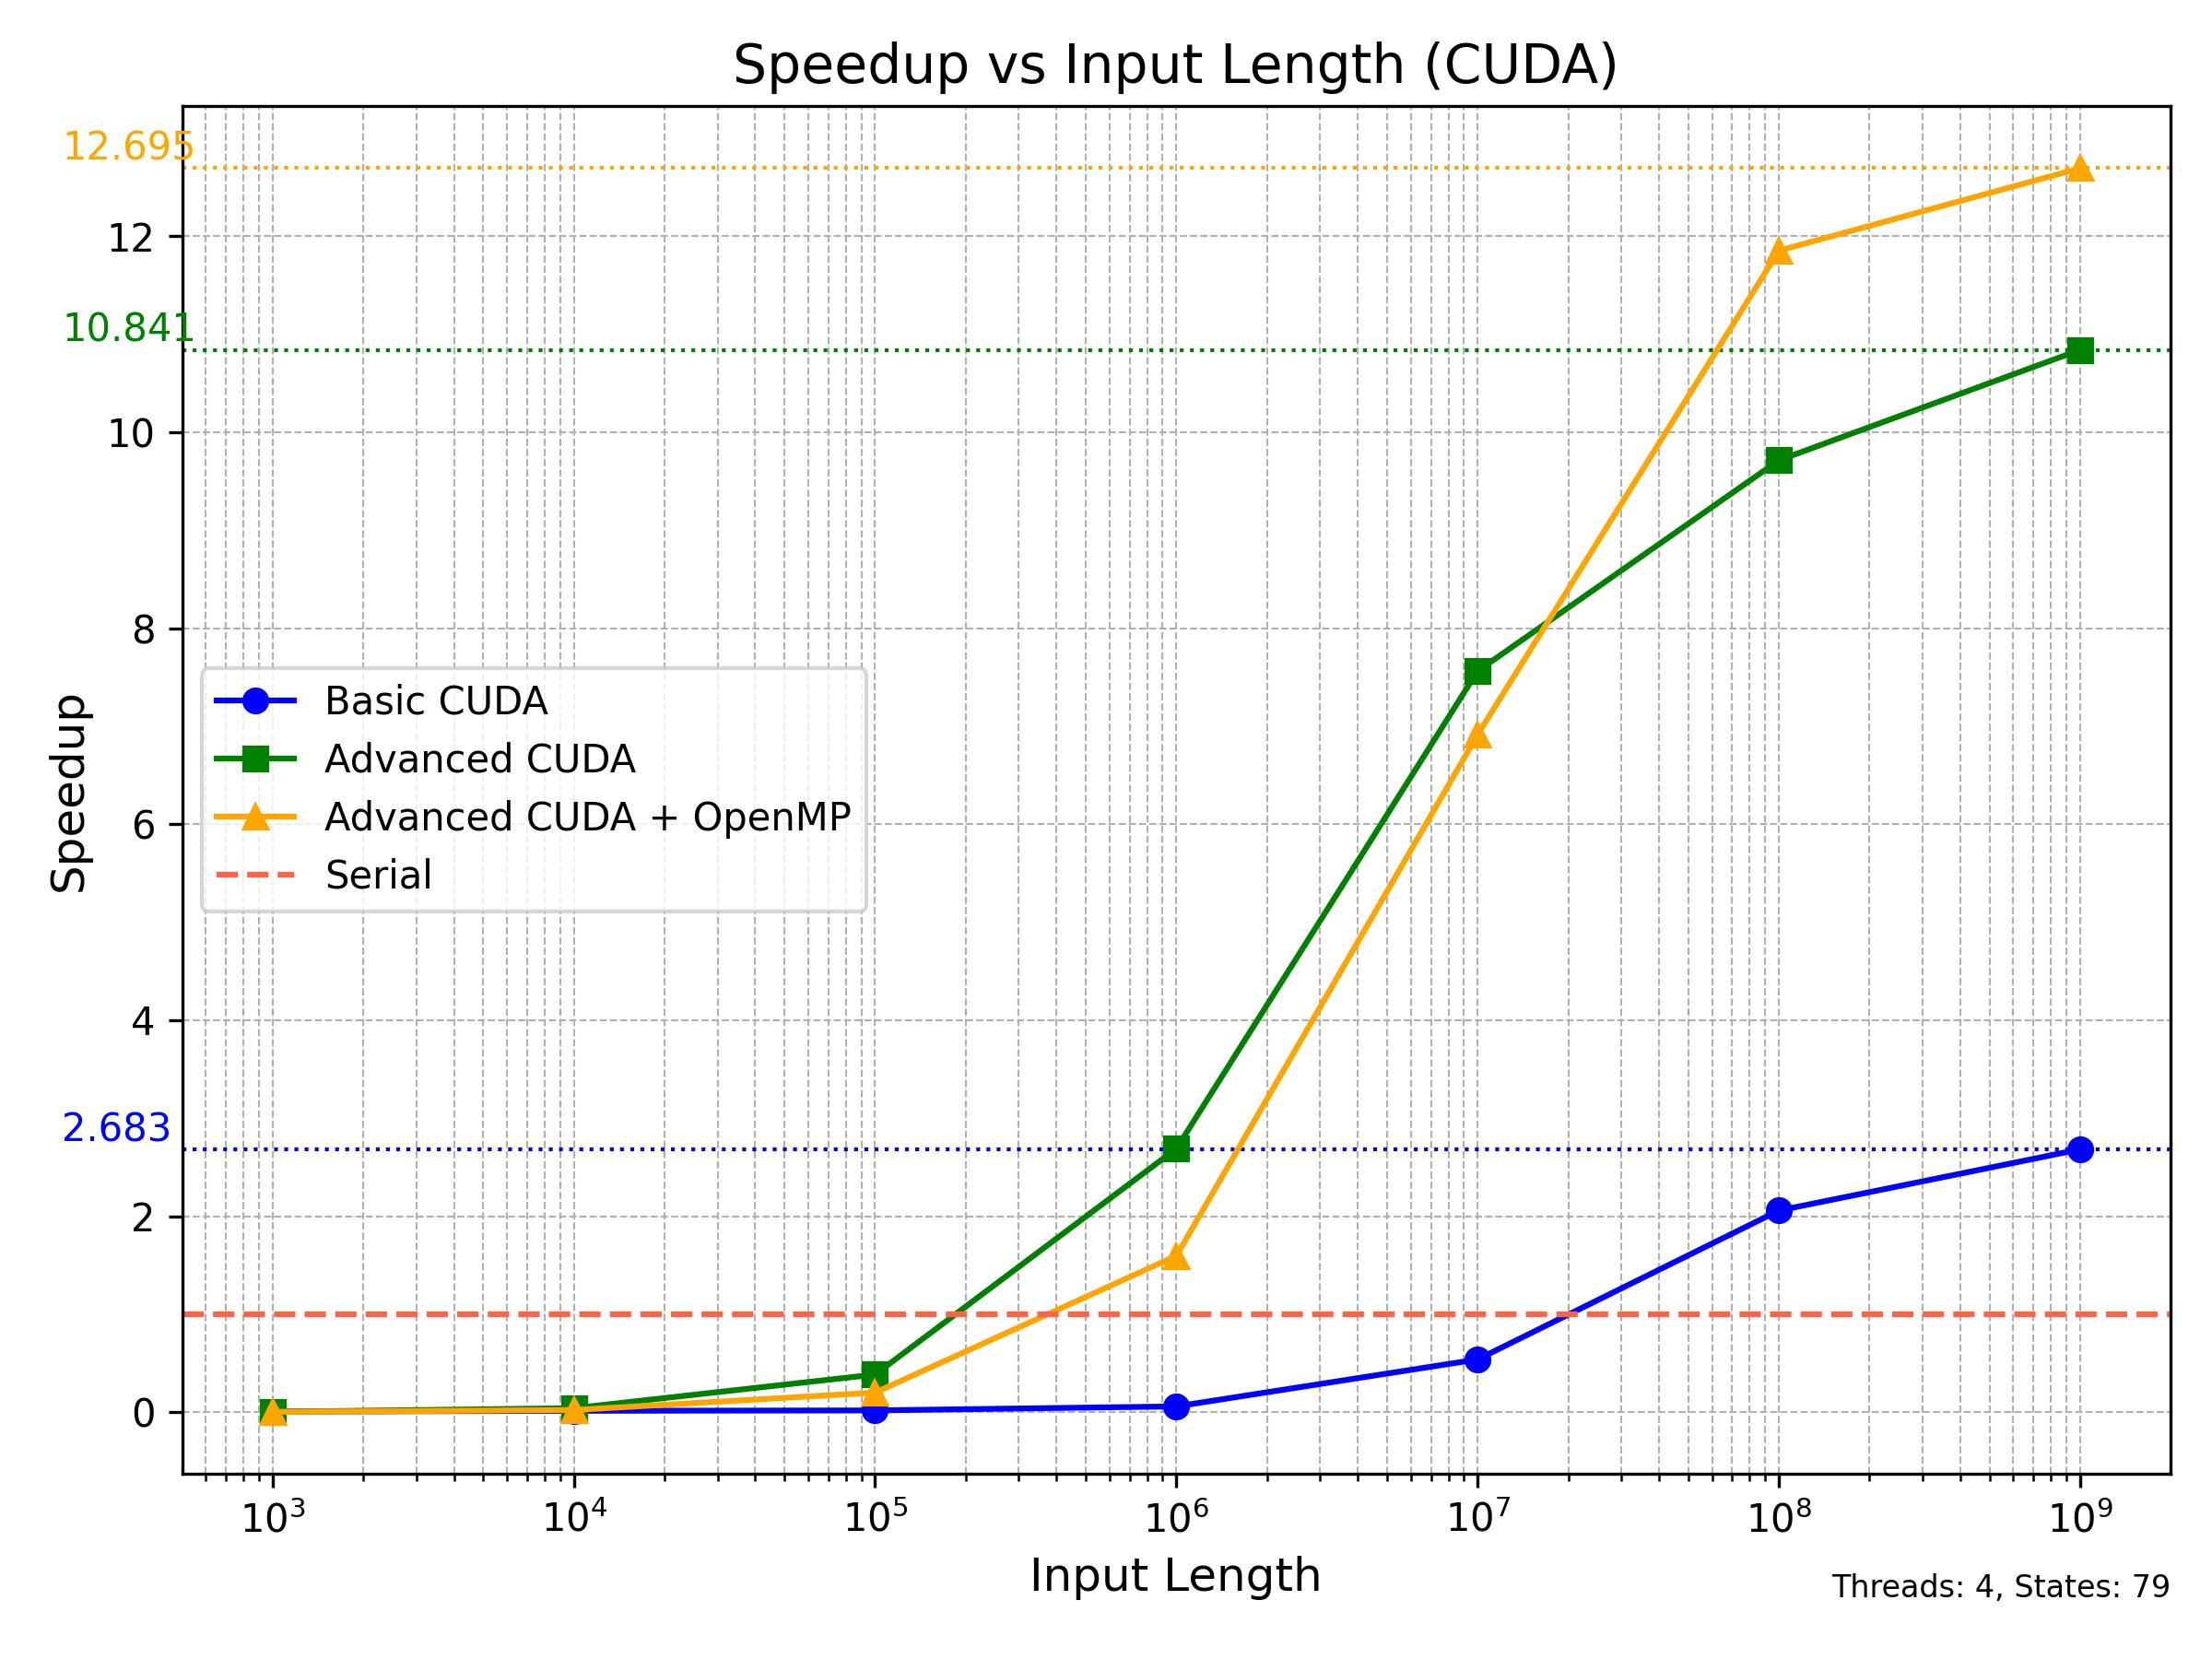
\includegraphics[width=\linewidth]{input_length_cuda}
		\caption{}
		\label{fig:SpeedupInputLengthCUDA}
	\end{subfigure}
	\begin{subfigure}{.33\textwidth}
		\centering
		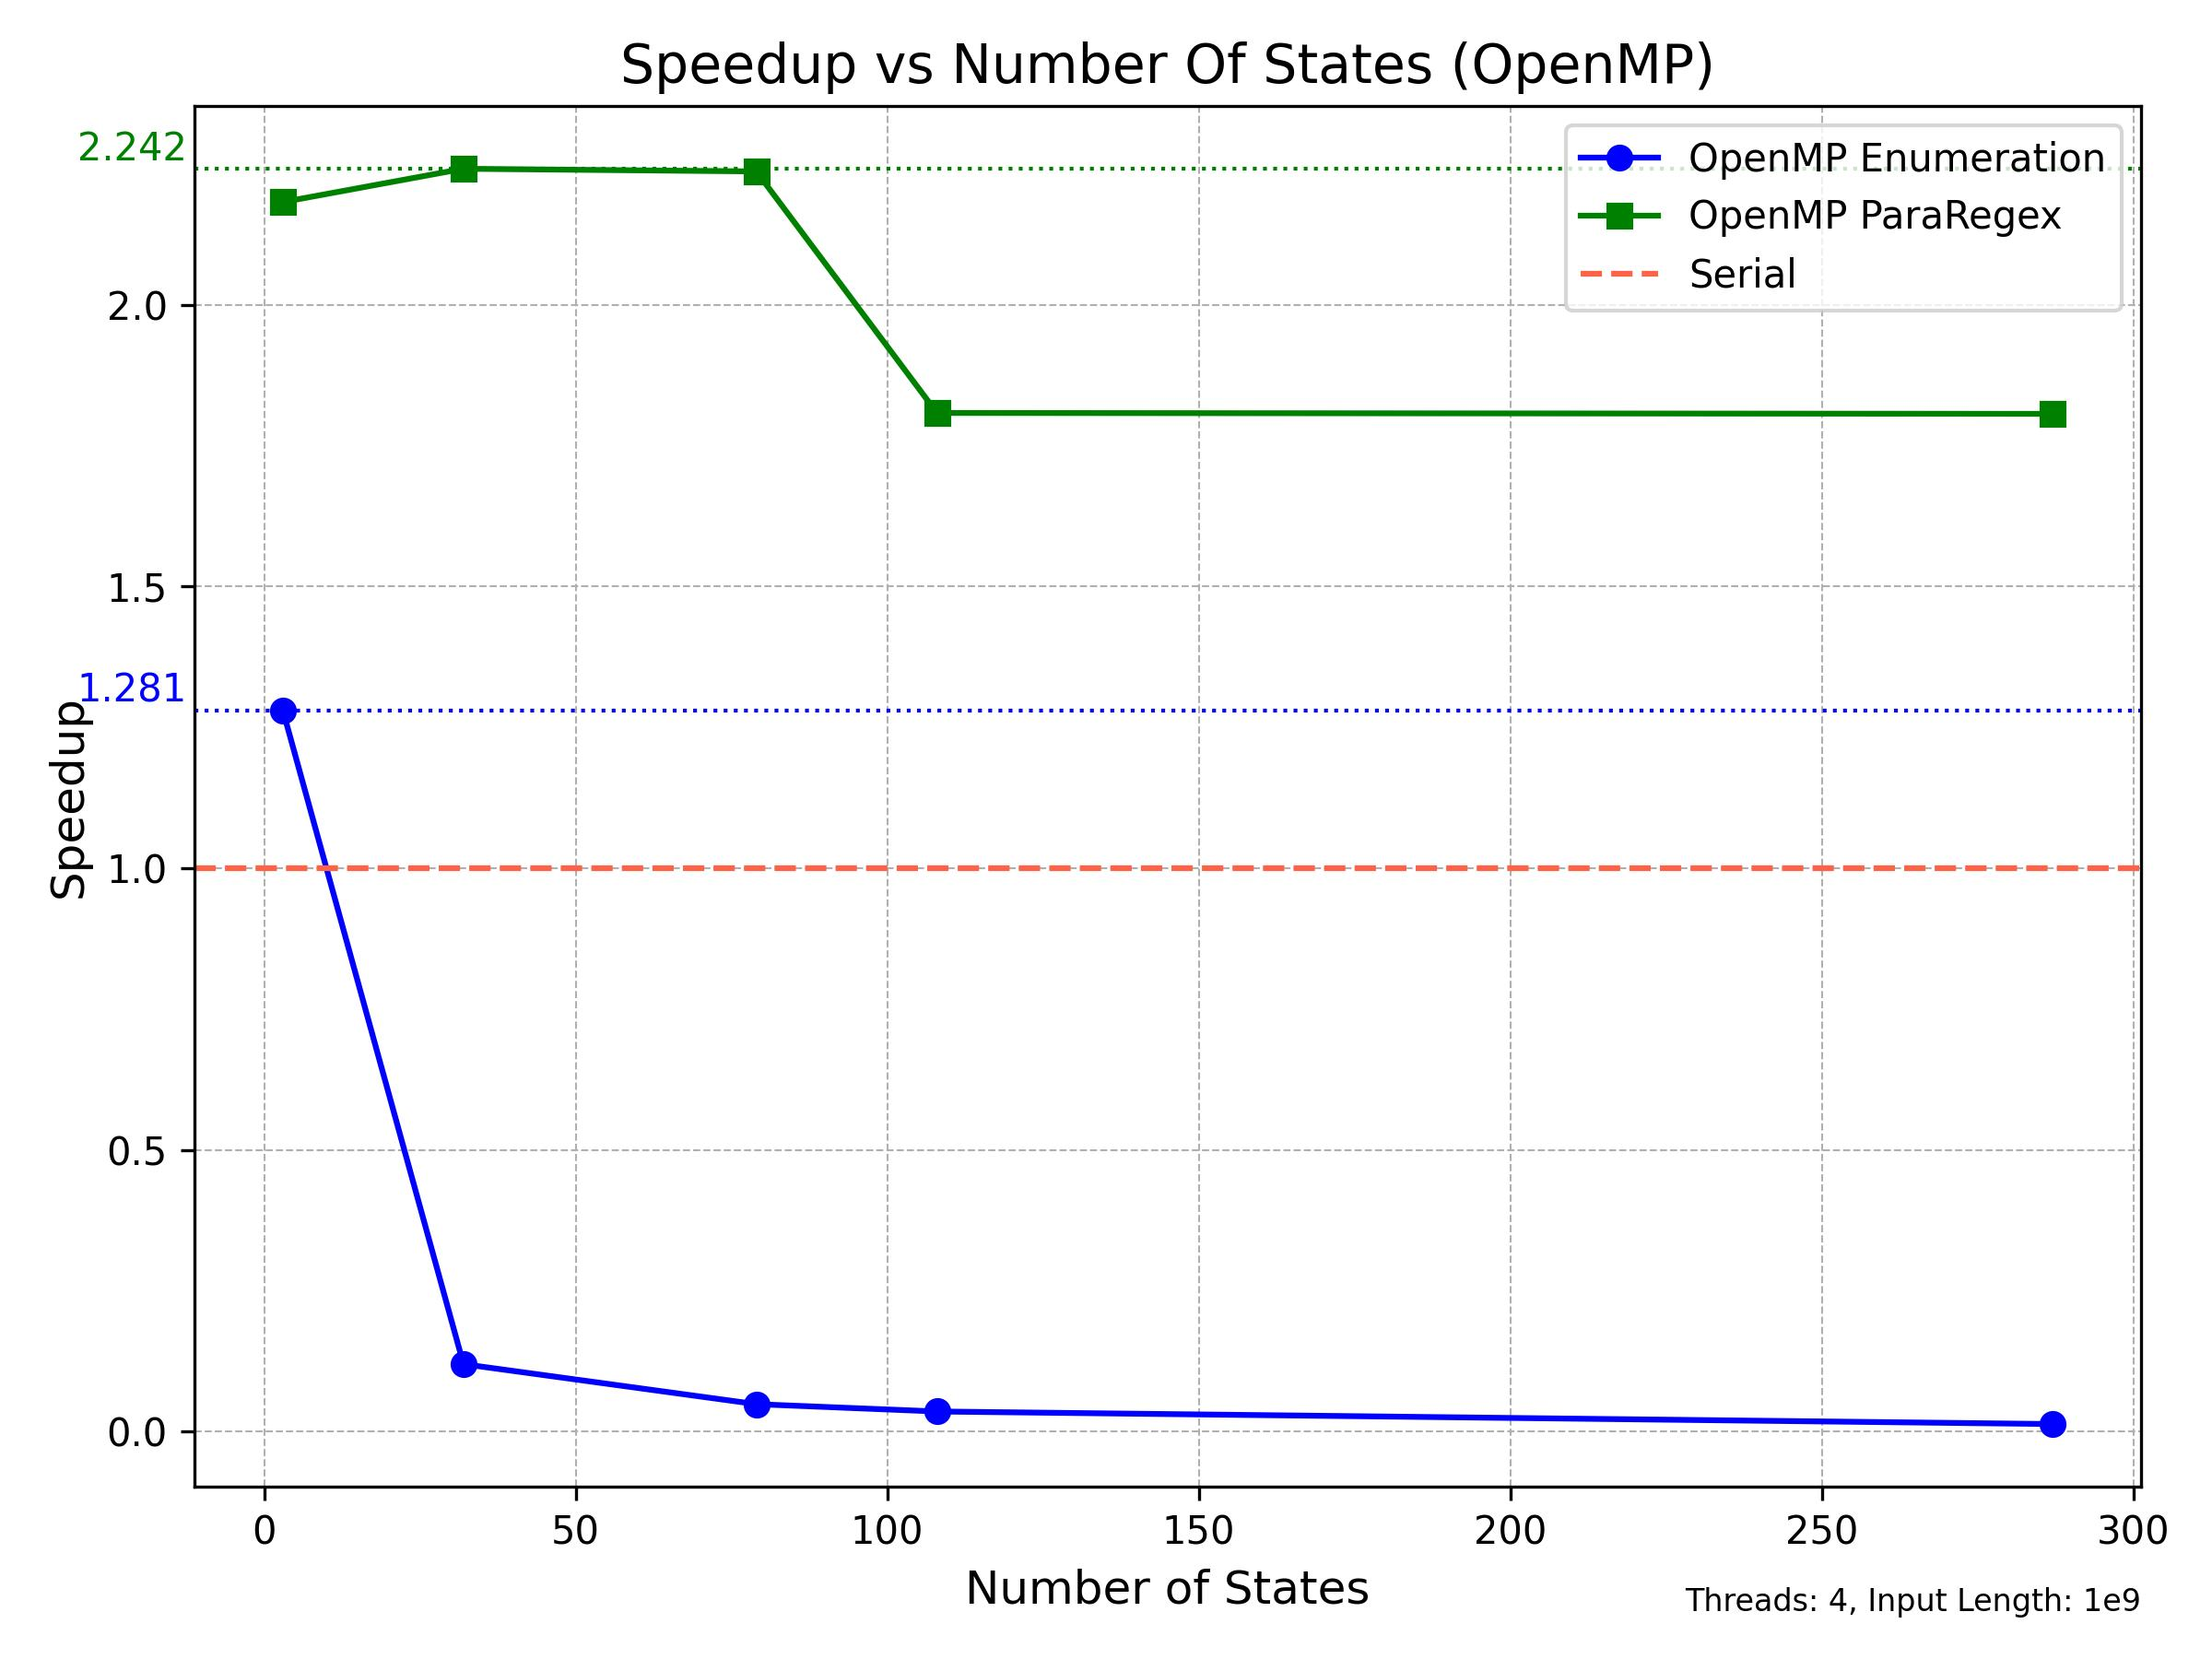
\includegraphics[width=\linewidth]{number_of_states_omp}
		\caption{}
		\label{fig:SpeedupStateOMP}
	\end{subfigure}
	\begin{subfigure}{.33\textwidth}
		\centering
		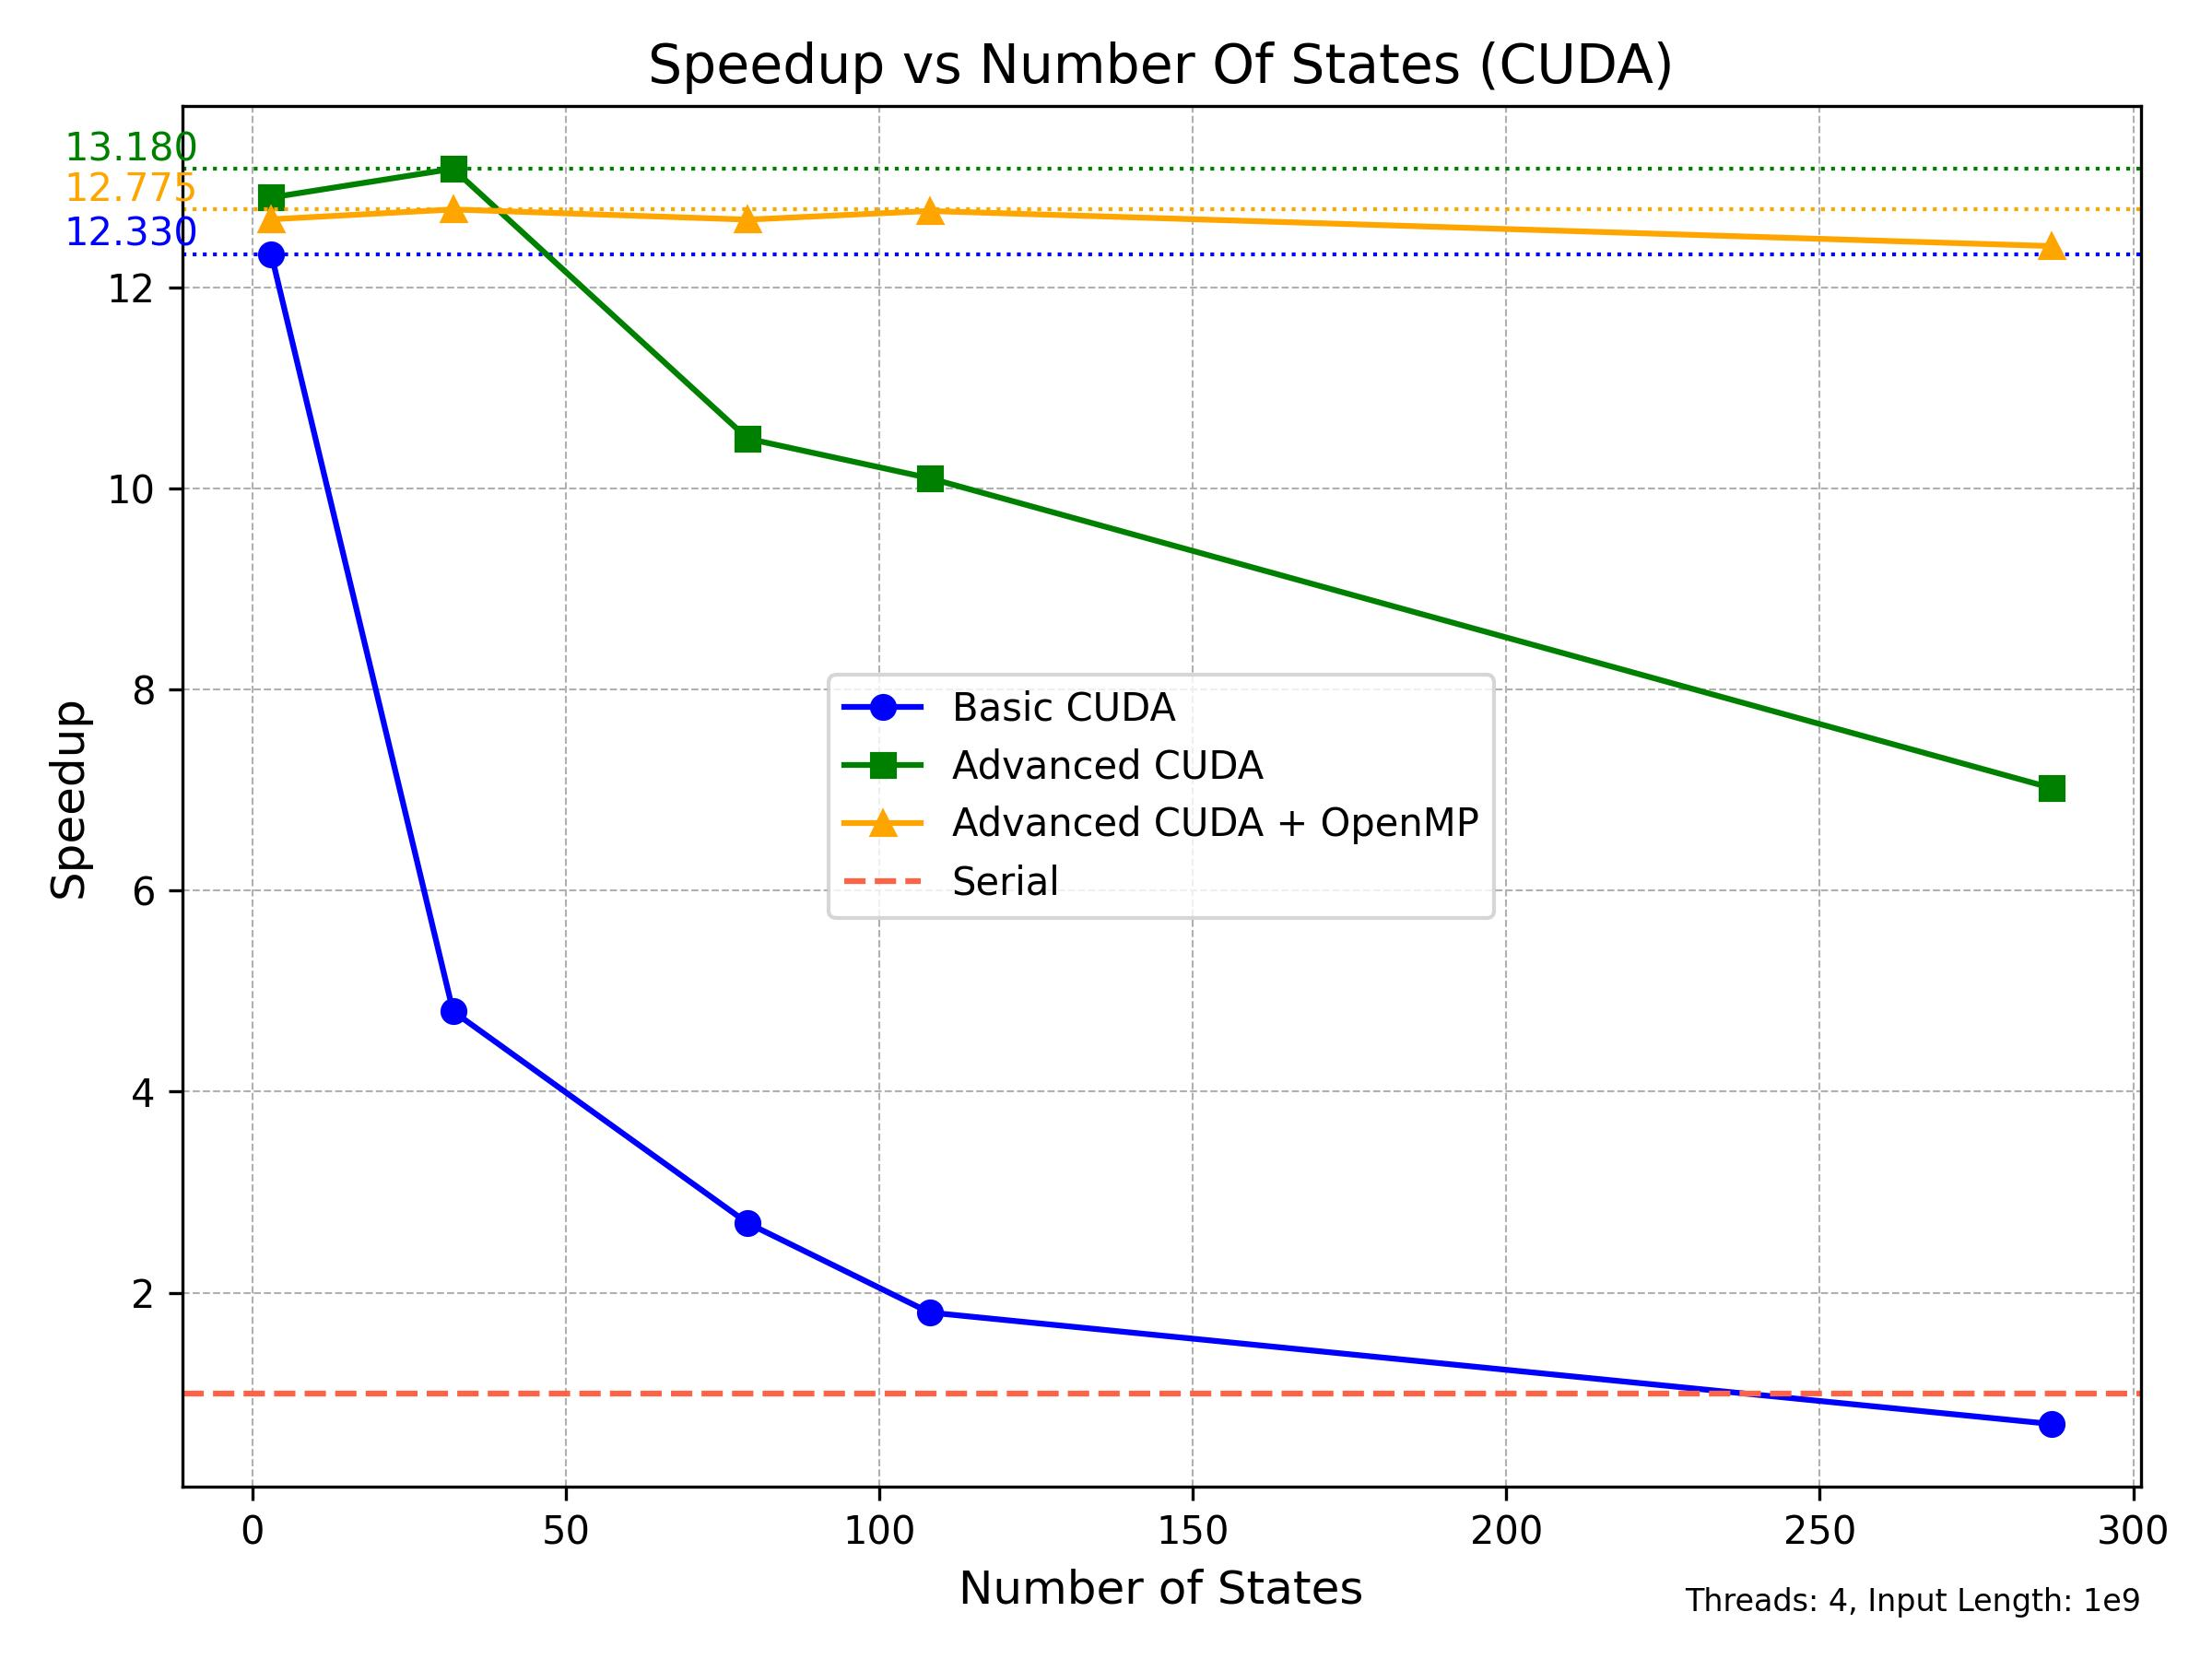
\includegraphics[width=\linewidth]{number_of_states_cuda}
		\caption{}
		\label{fig:SpeedupStateCUDA}
	\end{subfigure}
	\begin{subfigure}{.33\textwidth}
		\centering
		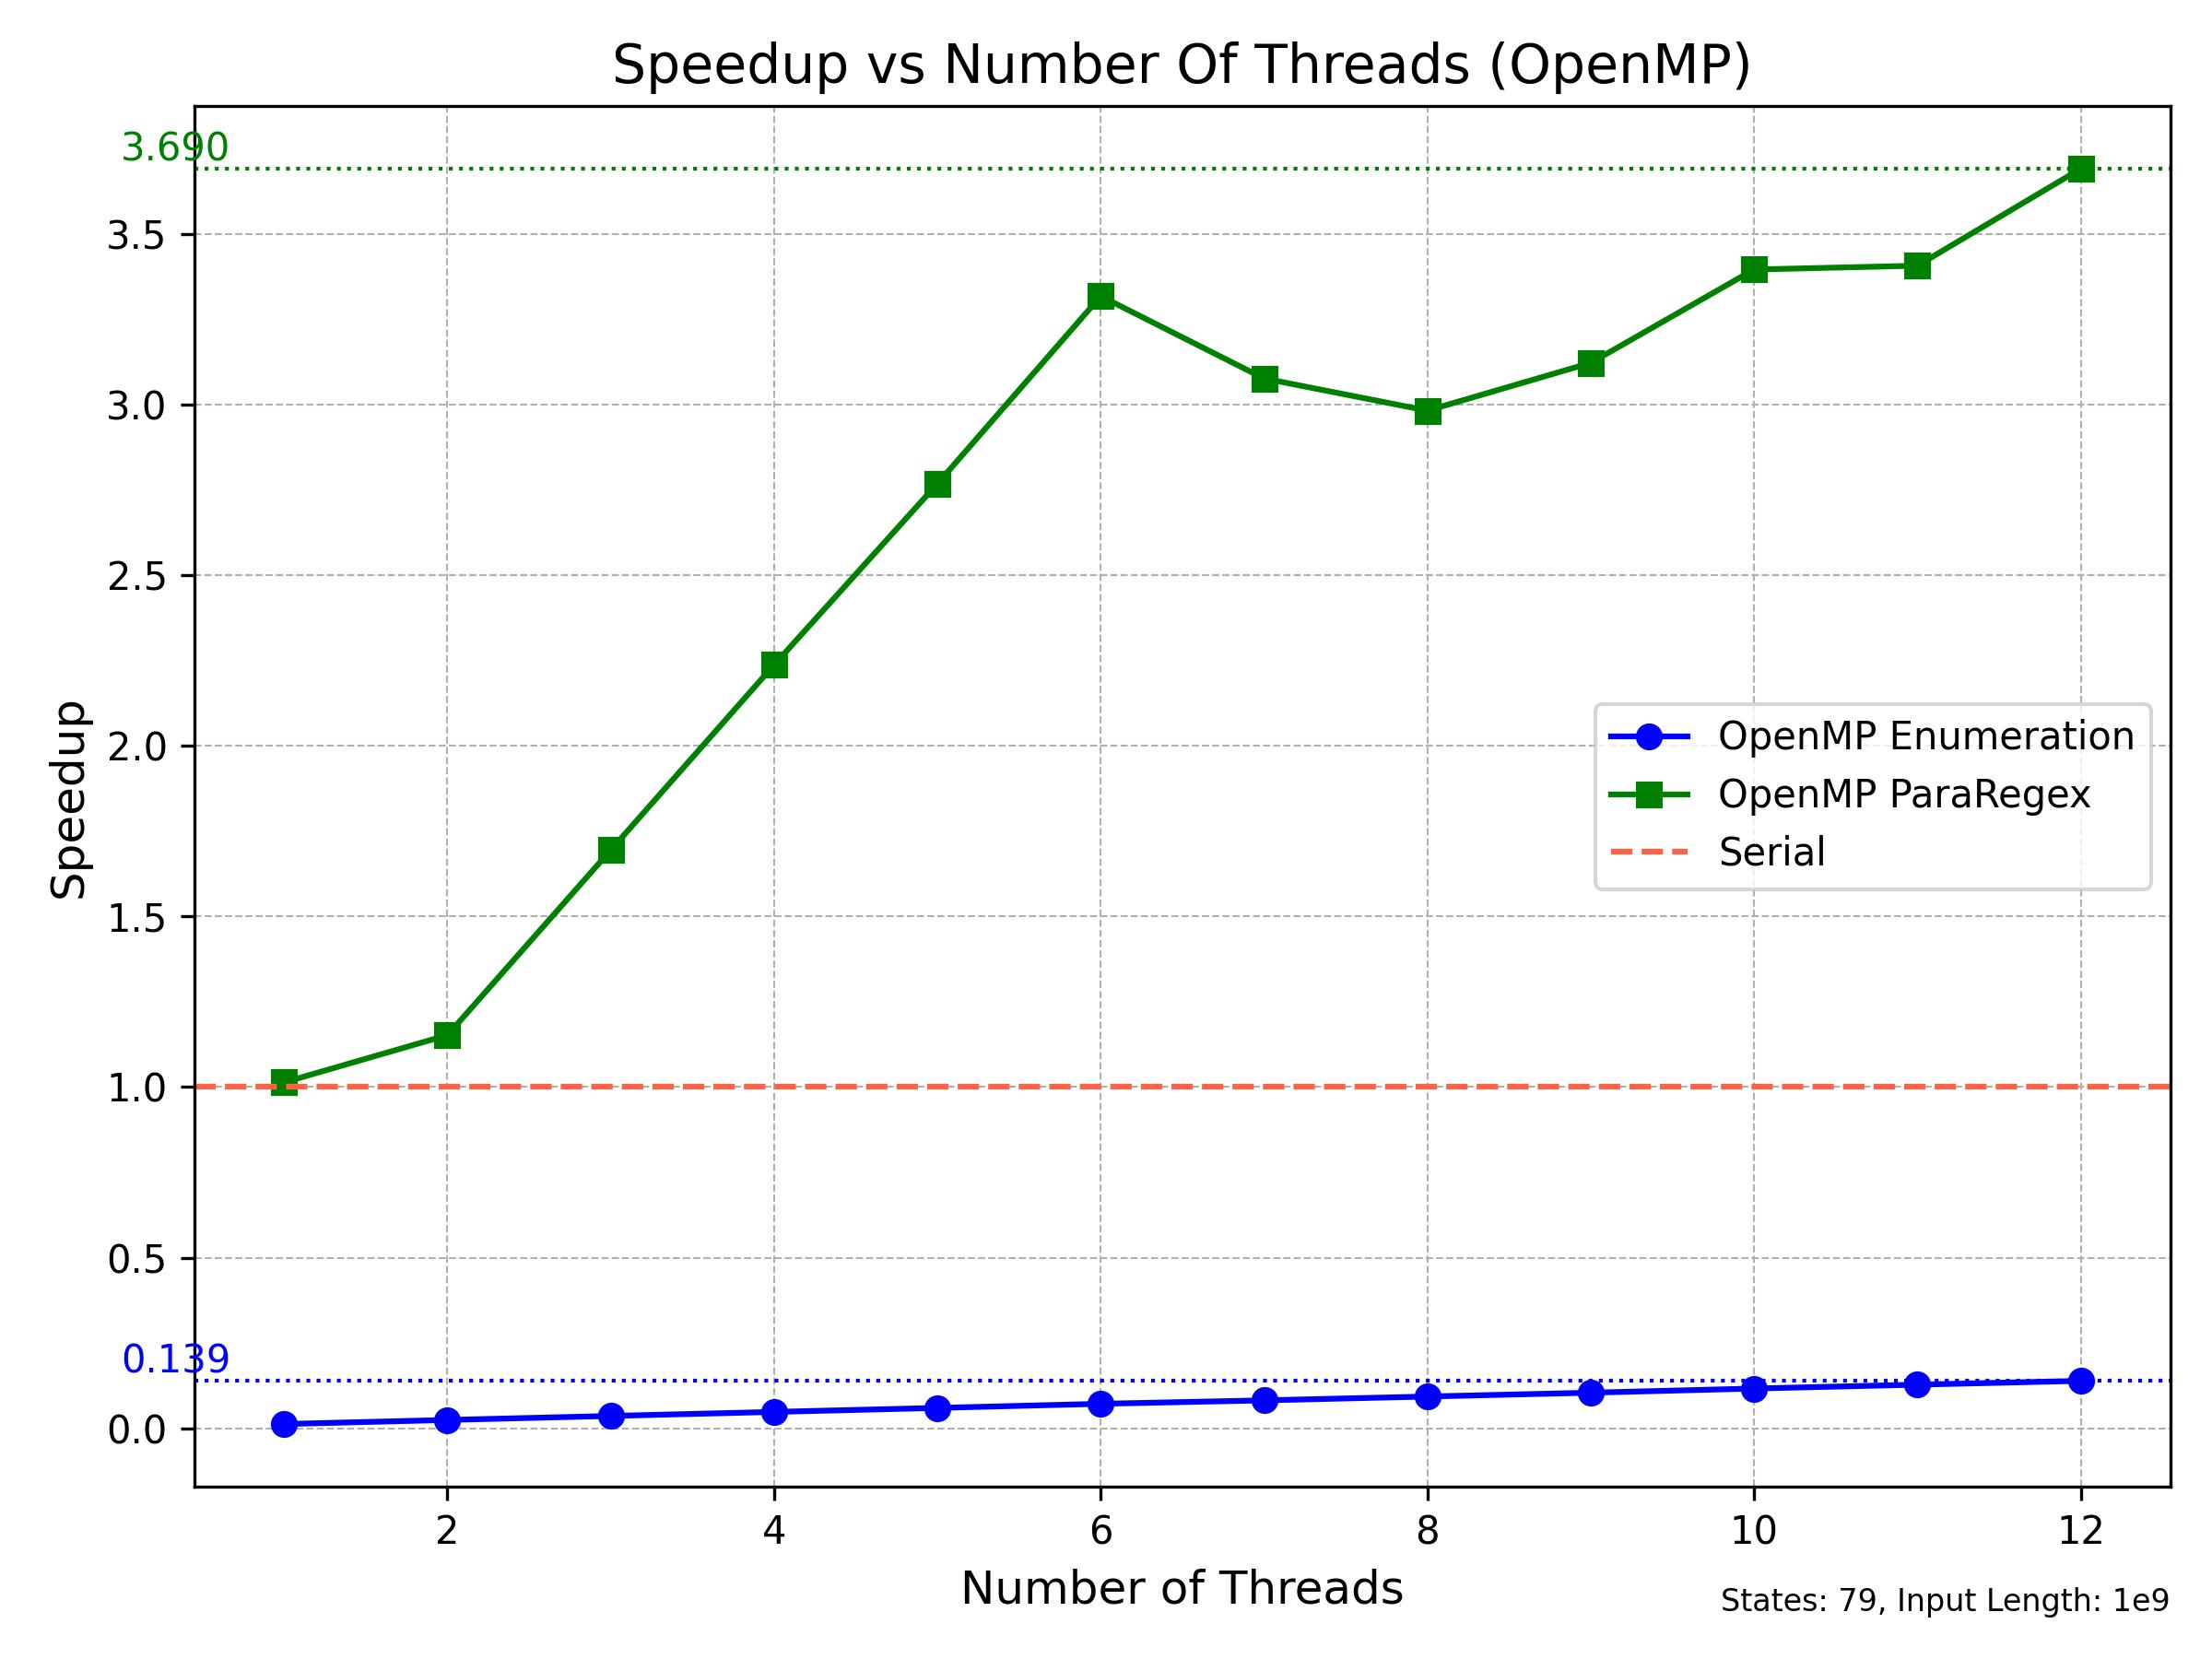
\includegraphics[width=\linewidth]{number_of_threads_omp}
		\caption{}
		\label{fig:SpeedupThread}
	\end{subfigure}
	\caption{Speedup against (a)(b) input length on OpenMP and CUDA, (c)(d) number of states on OpenMP and CUDA, and (e) on number of threads.}
	\label{fig:Speedup}
\end{figure*}

\subsection{Input Length}
The experiments reveal that increasing input length improves the relative performance of advanced methods. In Figure~\ref{fig:SpeedupInputLengthOMP}, we compare two OpenMP-based methods, where the x-axis represents the input length, ranging from $10^3$ to $10^9$, while the y-axis shows the speedup relative to the serial implementation.

As shown in Figure~\ref{fig:SpeedupInputLengthOMP}, the enumeration method experiences bottleneck due to their reliance on exhaustive state computations, leading to suboptimal performance compared to the baseline serial implementation. Specifically, the enumeration method performs significantly worse than the serial implementation due to the number of states exceeding the number of processors available. In contrast, Pararegex shows a clear trend of increasing speedup with longer input lengths. This is because, as input length $n$ grows, the latter terms in the complexity expression, namely $\log|P|$ and $|P|$, become negligible, allowing Pararegex to scale more effectively. Additionally, Pararegex demonstrates a substantial performance advantage over enumeration methods, highlighting that reducing active states significantly contributes to the observed speedup.

In Figure~\ref{fig:SpeedupInputLengthCUDA}, we compare three CUDA-based methods, where the speedup of these methods also increases as input length grows, for the same reasons discussed earlier. However, due to CUDA's higher number of processors, the speedups achieved are significantly greater than those observed in OpenMP-based approaches shown in Figure~\ref{fig:SpeedupInputLengthOMP}. Furthermore, the Advanced CUDA method improved the original method by reducing the overall number of memory accesses, resulting in a notable performance gain compared to the unoptimized enumeration approach. Among these, the Advanced CUDA + OpenMP method demonstrates an additional advantage, as it employs OpenMP to accelerate the reduction of active states. This leads to faster performance in the latter stages relative to the Advanced CUDA, which does not utilize OpenMP for this purpose.

\subsection{Number of States}
\label{sec:result_state}

We examined the impact of the DFA state count on OpenMP-based methods, as shown in Figure~\ref{fig:SpeedupStateOMP}. As expected, increasing the number of states introduces significant overhead due to state enumeration in OpenMP. In contrast, the OpenMP-based Pararegex method retains some speedup, although the performance results exhibit instability and variability. To better understand the effect of the active state mechanism, we define $|Q_{\text{active}}(n_p)|$ as the number of active states after processing $n_p$ inputs. Initially, $|Q_{\text{active}}(0)| = |Q|$, where $|Q|$ is the total number of states. As discussed in Theorem~\ref{thm:active_states}, as $n$ increases, $|Q_{\text{active}}(n_p)|$ decreases and eventually stabilizes at a minimum value, $q = \minof{|Q_{\text{active}}|} = |Q_{\text{active}}(n_{\minof{p}})|$, beyond which no further reduction occurs. We report the average of this minimum value, $\bar{q}$. Additionally, for each thread, we define $\rho = \left(\frac{n_{\minof{p}}}{n/|P|}\right)$ as the fraction of inputs required to reach the minimum active state count. The higher the $\rho$ is, the less portion of the matching process benefits from this active state mechanism. We analyze its minimum $\minof{\rho}$, maximum $\maxof{\rho}$, average $\bar{\rho}$, and standard deviation $\sigma_{\rho}$ across threads. The results summarized in Table~\ref{tab:StateReductionState} reveal two main trends:

\begin{enumerate}
	\item \textbf{Increased States Lead to More Reduction Loops:} As the number of states grows, additional state reduction loops are needed, increasing overhead.
	\item \textbf{Input Variability Across DFAs:} Different DFA configurations and input patterns cause fluctuations in overhead, resulting in unpredictable performance.
\end{enumerate}

\begin{table}[t]
	\caption{State Decrease Statistics Relative to DFA State Count}
	\label{tab:StateReductionState}
	\begin{tabular}{cccccc}
		\toprule
		$|Q|$ & $\bar{q}$ & $\bar{\rho}$ & $\sigma_{\rho}$ & $\minof{\rho}$ & $\maxof{\rho}$ \\
		\midrule
		3     & 1         & 0.00007      & 0.00007         & 0.00002        & 0.00015        \\
		32    & 1         & 0.00157      & 0.00225         & 0.00006        & 0.00417        \\
		79    & 1         & 0.01843      & 0.01058         & 0.01046        & 0.03044        \\
		108   & 1         & 0.38553      & 0.21499         & 0.17054        & 0.06089        \\
		287   & 1         & 0.38553      & 0.21499         & 0.17054        & 0.06089        \\
		\bottomrule
	\end{tabular}
\end{table}

We also analyzed the effect of the DFA state count on CUDA-based methods, as shown in Figure~\ref{fig:SpeedupStateCUDA}. As expected, increasing the number of states leads to a performance decline in CUDA enumeration. However, advanced CUDA techniques partially mitigate this overhead by leveraging optimized memory access. Despite this, performance still shows a downward trend. By combining state reduction with CUDA enumeration, we can leverage the extensive number of CUDA processors while minimizing state overhead, resulting in a more stable and consistent speedup.

\subsection{Number of Threads}
We next explored performance scaling with the number of threads using OpenMP. In Figure~\ref{fig:SpeedupThread}, the x-axis represents the number of threads (ranging from 1 to 12), and the y-axis displays the corresponding performance.

As shown in the figure, the enumeration method scales with the number of threads; however, due to the large number of states in the DFA, its performance remains slower than the serial implementation, even as the thread count increases.

The OpenMP-based Pararegex method, on the other hand, shows an increasing performance trend as the number of threads grows. However, the speedup is not linear. From the speedup analysis in Section~\ref{sec:result_state}, we observed that performance is strongly influenced by the number of active states, $|Q_{\text{active}}|$. To further investigate, we conducted the same analysis as in Section~\ref{sec:result_state}, but varied the number of threads, $|P|$. The results, shown in Table~\ref{tab:StateReductionThread}, combined with other observations, reveal the following key reasons for the observed non-linear speedup:

\begin{enumerate}
	\item \textbf{State Reduction Overhead:} Reducing the number of active states introduces overhead, preventing the method from achieving ideal speedup proportional to $|P|$.
	\item \textbf{Input and Partition Variability:} Different input segments and partitions lead to varying overheads for state reduction. In some cases, an unfavorable segment may result in higher active states, even if the segment is shorter.
	\item \textbf{Impact of Shorter Partitions:} As the number of threads increases, input partitions become smaller, magnifying the effects of ``\emph{bad loops}'' (where active states remain high). This limits the potential speedup, as the smaller partition sizes do not yield proportional performance improvements.
\end{enumerate}

\begin{table}[t]
	\caption{State Decrease Ratio Statistics Relative to Thread Count}
	\label{tab:StateReductionThread}
	\begin{tabular}{cccccc}
		\toprule
		$|P|$ & $\bar{q}$ & $\bar{\rho}$     & $\sigma_{\rho}$ & $\minof{\rho}$ & $\maxof{\rho}$ \\
		\midrule
		4     & 1         & 0.01843          & 0.01058         & 0.01046        & 0.03044        \\
		6     & 1         & 0.02139          & 0.01690         & 0.00435        & 0.04567        \\
		8     & 1         & 0.02518          & 0.02396         & 0.02396        & 0.06089        \\
		10    & 1         & 0.01651          & 0.02604         & 0.00009        & 0.07611        \\
		12    & 1         & \textbf{0.04787} & 0.04142         & 0.00333        & 0.12846        \\
		\bottomrule
	\end{tabular}
\end{table}

\section{Related work}
Recent advancements in parallel regular expression matching have leveraged deterministic finite automata (DFA) to optimize pattern recognition tasks. For instance, Memeti et al. \cite{PaREM} introduced the PaREM algorithm, which also splits the input into $|P|$ parts, but it excludes all the states that the automaton has no outgoing or incoming transitions for the specified characters because calculating the possible routes from each state of the automaton are too time-consuming and memory-expensive. However, this method works better for smaller regular expression rulesets and doesn't work well for larger rulesets.

On the other hand, traditional approaches often face the trade-off between computational efficiency and memory usage. For instance, DFA-based methods, while offering faster matching speeds, suffer from state explosion, significantly increasing memory requirements. To address these issues, Yang Yi-Hua et al. \cite{Semi-Deterministic-Finite-Automata} introduced the Semi-Deterministic Finite Automata. This hybrid model balances the computational efficiency of DFAs with the conciseness of NFAs.

We also find many existing methods for parallelizing regular expression matching, each focusing on improving the efficiency of state machine models. In Simultaneous Finite Automaton (SFA)\cite{Simultaneous-Finite-Automaton}, Sinya et al. introduced a parallelizable automaton that extends traditional finite automata by simulating transitions from all states simultaneously, achieving over 10x speedups compared to sequential DFA-based approaches. In \cite{BSP}, Tachon and Thibaut transform regular expressions into a parallel form (BSPRE), which is then converted into parallel automata (BSPA), enabling more efficient parallel matching, particularly with small numbers of processors. In Nondeterministic Bit Vector Automata (NBVA)\cite{NBVA}, Le Glaunec et al. introduced a model designed for efficiently handling regexes with bounded repetition, achieving matching times independent of repetition bounds. Unlike the above approaches, our method builds upon the basic DFA model and takes advantage of the state transition properties. However, we may incorporate the aforementioned advanced models for further improvements, due to the generality of our methods built upon the basic DFA.

There is another popular optimization direction in parallel regex matching that focuses on utilizing specific hardware platforms for further improvements in algorithm performance. In \cite{FPGA}, the authors integrated Field-Programmable Gate Arrays (FPGAs) within a data processing framework, showcasing notable improvements in processing efficiency and match accuracy, particularly for complex regular expressions in network security and database applications. In \cite{semi}, the authors proposed a massively parallel, non-von Neumann semiconductor architecture, purpose-built for automata processing, which significantly outperformed high-performance FPGA-based implementations for complex regular expression matching tasks. In \cite{HybridSA}, the authors explored bit-parallel memory access patterns, resulting in a significant increase in throughput on the specific HybridSA engine for which the method was designed. This approach is particularly suitable for scenarios where hardware-level optimizations can enhance performance.
In contrast, our work currently explores parallel regex algorithms on the OpenMP and CUDA frameworks, but it is not specialized for a specific hardware parallel platform. We focus on leveraging general parallel programming models to improve performance on multi-core CPUs and GPUs. However, the potential to optimize our approach by incorporating hardware-specific optimizations, such as FPGA-based accelerators or custom architectures designed for automata processing, represents an exciting direction for future research.

\section{Conclusions}

This study presented a comprehensive approach to parallelizing DFA-based regex matching, addressing the limitations of traditional enumeration methods. By incorporating active state tracking and leveraging advanced CUDA and OpenMP techniques, the proposed methods achieve substantial speedups across various configurations. Experimental results highlight the effectiveness of Pararegex in reducing computational overhead and the potential of CUDA optimizations for leveraging massive parallelism. Future work could explore further integration of hybrid CPU-GPU approaches and adaptive algorithms for dynamically adjusting active state management based on input characteristics.

% references
\bibliographystyle{ACM-Reference-Format}
\bibliography{pp-final}

\end{document}
